\documentclass{standalone}

\usepackage{tikz}
\usetikzlibrary{automata, arrows.meta, positioning}

\begin{document}
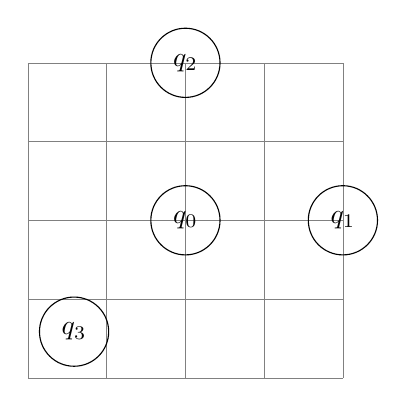
\begin{tikzpicture} [node distance = 2 cm, on grid] % on grid = distances between center points
  \draw [help lines] (-2,2) grid (2,-2);

  % States
  \node (q0) [state] {$q_{0}$};
  \node (q1) [state, right = of q0] {$q_{1}$};
  \node (q2) [state, above = of q0] {$q_{2}$};
  \node (q3) [state, below left = of q0] {$q_{3}$};
\end{tikzpicture}
\end{document}
